\documentclass[a4paper,14pt]{extreport}
	\usepackage[left=1.5cm,right=1.5cm,
	    top=1.5cm,bottom=2cm,bindingoffset=0cm]{geometry}
	\usepackage{scrextend}
	\usepackage[T1,T2A]{fontenc}
	\usepackage[utf8]{inputenc}
	\usepackage[english,russian,ukrainian]{babel}
	\usepackage{tabularx}
	\linespread{1.5}
	\usepackage{amssymb}
	\usepackage{color}
	\usepackage{amsmath}
	\usepackage{mathrsfs}
	\usepackage{listings}
	\usepackage{graphicx}
	\graphicspath{ {./images/} }
	\usepackage{lipsum}
	\usepackage{xcolor}
	\usepackage{hyperref}
	\usepackage{tcolorbox}
	\usepackage{tikz}
	\usepackage[framemethod=TikZ]{mdframed}
	\usepackage{wrapfig,boxedminipage,lipsum}
	\mdfdefinestyle{MyFrame}{%
	linecolor=blue,outerlinewidth=2pt,roundcorner=20pt,innertopmargin=\baselineskip,innerbottommargin=\baselineskip,innerrightmargin=20pt,innerleftmargin=20pt,backgroundcolor=gray!50!white}
	 \usepackage{csvsimple}
	 \usepackage{supertabular}
	\usepackage{pdflscape}
	\usepackage{fancyvrb}
	%\usepackage{comment}
	\usepackage{array,tabularx}
	\usepackage{colortbl}
\usepackage{floatrow}   %я вот это пакет тебе подключил, шо можно было \TopFloatBoxes\CenterFloatBoxes писать
	\usepackage{varwidth}
	\tcbuselibrary{skins}
	\usepackage{fancybox}
	\usepackage{multicol}
	\usepackage{multirow}
	\usepackage{pgfplots}
	\pgfplotsset{compat=1.9}


	\usepackage{tikz}
	\usepackage[framemethod=TikZ]{mdframed}
	\usepackage{xcolor}
	\usetikzlibrary{calc}
	\makeatletter
	\newlength{\mylength}
	\xdef\CircleFactor{1.1}
	\setlength\mylength{\dimexpr\f@size pt}
	\newsavebox{\mybox}
	\newcommand*\circled[2][draw=blue]{\savebox\mybox{\vbox{\vphantom{WL1/}#1}}\setlength\mylength{\dimexpr\CircleFactor\dimexpr\ht\mybox+\dp\mybox\relax\relax}\tikzset{mystyle/.style={circle,#1,minimum height={\mylength}}}
	\tikz[baseline=(char.base)]
	\node[mystyle] (char) {#2};}
	\makeatother

	\definecolor{ggreen}{rgb}{0.4,1,0}
	\definecolor{rred}{rgb}{1,0.1,0.1}
	\definecolor{amber}{rgb}{1.0, 0.75, 0.0}
	\definecolor{babyblue}{rgb}{0.54, 0.81, 0.94}
	\definecolor{amethyst}{rgb}{0.6, 0.4, 0.8}

	\usepackage{float}
	\usepackage{wrapfig}
	\usepackage{framed}
	%for nice Code{
	\lstdefinestyle{customc}{
	  belowcaptionskip=1\baselineskip,
	  breaklines=true,
	  frame=L,
	  xleftmargin=\parindent,
	  language=C,
	  showstringspaces=false,
	  basicstyle=\small\ttfamily,
	  keywordstyle=\bfseries\color{green!40!black},
	  commentstyle=\itshape\color{purple!40!black},
	  identifierstyle=\color{blue},
	  stringstyle=\color{orange},
	}
	\lstset{escapechar=@,style=customc}
	%}
%----------------------------------------%----------------------------------------%----------------------------------------%----------------------------------

\begin{document}
\pagecolor{white}

%----------------------------------------1
\newtcbox{\xmybox}[1][red]{on line, arc=7pt,colback=#1!10!white,colframe=#1!50!black, before upper={\rule[-3pt]{0pt}{10pt}},boxrule=1pt, boxsep=0pt,left=6pt,right=6pt,top=2pt,bottom=2pt}

\begin{titlepage}
  \begin{center}
    \large
    Національний технічний університет України \\ "Київський політехнічний інститут імені Ігоря Сікорського"


    Факультет Електроніки

    Кафедра мікроелектроніки
    \vfill

    \textsc{ЗВІТ}\\

    {\Large Про виконання РГР\\
      з дисципліни: «Схемотехніка-1»\\[1cm]

        «Синтез активних RC-фільтрів»


	    }
	  \bigskip
	\end{center}
	\vfill

	\newlength{\ML}
	\settowidth{\ML}{«\underline{\hspace{0.4cm}}» \underline{\hspace{2cm}}}
	\hfill
	\begin{minipage}{1\textwidth}
	Виконавець:\\
	Студент 3-го курсу \hspace{4cm} $\underset{\text{(підпис)}}{\underline{\hspace{0.2\textwidth}}}$  \hspace{1cm}А.\,С.~Мнацаканов\\
	\vspace{1cm}

	Перевірила: \hspace{6.1cm} $\underset{\text{(підпис)}}{\underline{\hspace{0.2\textwidth}}}$  \hspace{1cm}Г.\,С.~Порева\\

	\end{minipage}

	\vfill

	\begin{center}
	2021
	\end{center}
\end{titlepage}


\begin{center}\textbf{Завдання}\end{center}\par
\begin{enumerate}
	\item Визначити параметри специфікації для синтезу активного RC-фільтра. Обрати тип
	фільтру у відповідності до варіанту табл. 1, тип апроксимації АЧХ обрати у відповідності
	до табл. 2, числові параметри відповідно до табл. 3.
	\item  Визначити необхідний порядок фільтру та записати аналітичний вираз для функції
	передачі фільтру у загальному вигляді.
	\item  Записати аналітичний вираз функції передачі фільтру у вигляді послідовно з’єднаних
	ланок другого порядку в загальному вигляді.
	\item  Розрахувати коефіцієнти функції передачі фільтру.
	\item  Обрати структури фільтрів для реалізації ланок другого порядку.
	\item  Розробити принципову електричну схему активного RC-фільтру для кожної ланки другого
	порядку (провести аналітичний розрахунок секцій другого порядку, провести розрахунки
	номіналів схеми, обрати елементну базу).
	\item  Оформити повну схему електричну принципову розробленого фільтра у відповідності до
	вимог ЕСКД.
	\item  Провести аналіз розробленої схеми. Побудувати АЧХ та ФЧХ розробленого фільтра.
	Впевнитися у відповідності параметрів розробленого фільтра вимогам специфікації.
\end{enumerate}
\newpage

\begin{center}
\fbox{1}
\end{center}
	Тип активного RC-фільтра: $ N_1 = mod(4+5,4) = 1$;\\
	Тип апроксимації АЧХ: $N_2 = mod(mod(5\cdot 4+3\cdot 5, 7), 3) = 0; \Rightarrow $  Батерворта;\\
	Коефіцієнт передачі у смузі пропускання: $G_{ain}$=3 дБ;\\
	$f_p$ = 4 кГц;\\
	$f_s$ = 1.33 кГц;\\
	Рівень пульсації у смузі пропускання: $R_p$=6 дБ;\\
	Мінімальне подавлення у смузі затримки: $R_s$=22 дБ;\\

\begin{center}
\fbox{2}
\end{center}
	\begin{center}
	\textbf{Код на matlab}
	\end{center}
	\lstinputlisting[language=Octave]{cod.txt}
\newpage
Функція передачі в загальному вигляді виглядає наступним чином:
\begin{equation}
K_U(p)=\dfrac{B(p)}{A(p)}=\dfrac{b(1)\cdot p^n+b(2)\cdot p^{n-1}+...+b(n+1)}{a(1)\cdot p^n+a(2)\cdot p^{n-1}+...+a(n+1)}.
\end{equation}

\begin{center}
\fbox{3}
\end{center}

Запишемо вирази $K_U(p)$ послідовно з'єднаних ланок:
	\begin{equation}\label{two}
	K_{U_{\sum}}(p)=K_{U1}(p)K_{U2}(p)=-\dfrac{R_4}{R_3}\times-\dfrac{C_1C_3\cdot p^2}{C_2C_3\cdot p^2+G_2(C_1+C_2+C_3)\cdot p+G_2G_1}
	\end{equation} 

	Модифікуємо формулу \eqref{two} наступним чином:
	\begin{equation}\label{eq}
	K_U(p)=\dfrac{R_4}{R_3}\times\dfrac{C_1C_3\cdot p^2}{C_2C_3\left[p^2+\dfrac{G_2(C_1+C_2+C_3)}{C_2C_3}\cdot p+\dfrac{G_2G_1}{C_2C_3}\right]}
	\end{equation}


\begin{center}
\fbox{4}
\end{center}

\begin{figure}[!h]\TopFloatBoxes\CenterFloatBoxes
	          {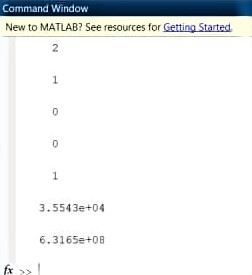
\includegraphics[width=0.3\textwidth]{prog_result}}
	           \caption{Результат роботи програми}
\end{figure}


Таким чином знаходимо порядку фiльтра(2) та коефiцiєнти функцiї \\ передачi(1,0,0,1,$3,5\cdot 10^4, 6,3\cdot 10^8$). 
	$$ K_u(p) = G_{ain}\cdot \dfrac{p^2}{p^2+3,5\cdot 10^4\cdot p+6,3\cdot10^8}, $$
	де $G_{ain} = 3 $ дБ = 1,413, тоді
\begin{equation}\label{tre}
	 K_u(p) = 1,4\cdot \dfrac{p^2}{p^2+3,5\cdot 10^4\cdot p+6,3\cdot10^8}
\end{equation}
\newpage
\begin{center}
\fbox{5}
\end{center}

	Підберемо таку структуру фільтра аби вона задовольняла нашому виразу для $K_U(p)$. Відповідно до формули \eqref{two} для цього зручно буде обрати каскадне з'єднання {\bf схеми Рауха} інвертуючого ФВЧ-2 порядку та інвертуючого масштабуючого підсилювача, аби забезпечити необхідне підсилення.

	\begin{figure}[h]
	           {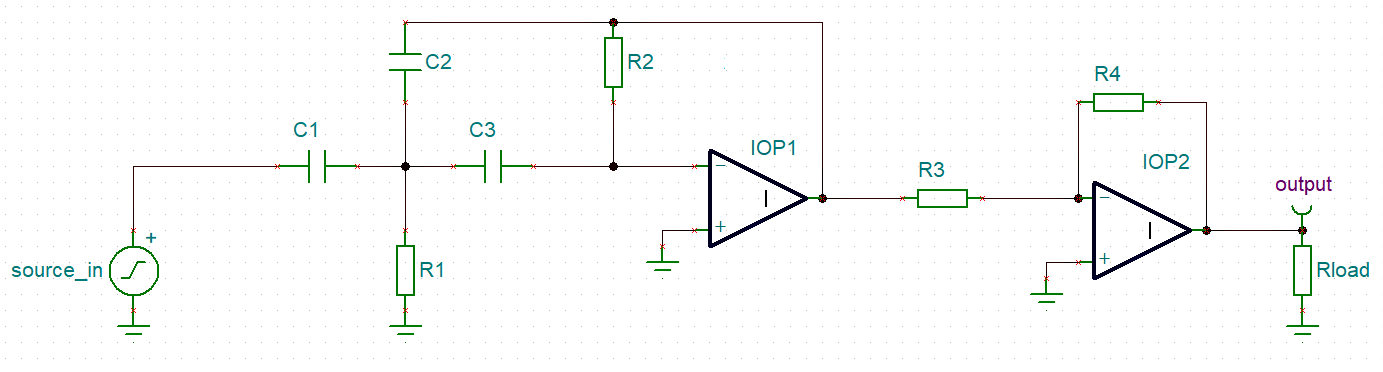
\includegraphics[width=\textwidth]{rauh}}
	           \caption{Схема рауха інвертуючого ФВЧ-2 та масштабуючого підсилювача}
	\end{figure}
	

\begin{center}
\fbox{6}
\end{center}
	
Спростивши вираз \eqref{eq} та об'єднавши його з \eqref{tre}, маємо:

	\begin{equation}
	\boxed{
	\begin{aligned}
	K_U(p)=\left(\dfrac{R_4}{R_3}\cdot\dfrac{C_1}{C_2}\right)\times\dfrac{p^2}{p^2+\dfrac{G_2(C_1+C_2+C_3)}{C_2C_3}\cdot p+\dfrac{G_2G_1}{C_2C_3}}\\[0.5cm]
	K_U(p)=1,413\times\dfrac{p^2}{p^2+3,5543\cdot{10^4}\cdot p+6,3165\cdot{10^8}}
	\end{aligned}}
	\end{equation}

Прирівняємо між собою коефіцієнти, записавши наступну систему рівнянь:

	\begin{equation*}
	\begin{cases}
	\dfrac{R_4}{R_3}\cdot\dfrac{C_1}{C_2}=1,413\\[0.5cm]
	\dfrac{G_2(C_1+C_2+C_3)}{C_2C_3}=3,5543\cdot{10^4}\\[0.5cm]
	\dfrac{G_2G_1}{C_2C_3}=6,3165\cdot{10^8}
	\end{cases}
	\end{equation*}
\newpage
	\begin{itemize}
	\item нехай $C_1=C_2=C_3=C=1$ нФ.
	\item з другого рівняння знаходимо $G_2$ як:
	\begin{center}
	$G_2=\dfrac{3,5543\cdot{10^4}\times C^2}{3C}=\dfrac{3,5543\cdot{10^4}\times \left(10^{-9}\right)^2}{3\cdot{10^{-9}}}=1,185\cdot{10^{-5}}$ См.
	\end{center}
	\item з третього рівняння знаходимо $G_1$ як:
	\begin{center}
	$G_1=\dfrac{6,3165\cdot{10^8}\times{C^2}}{G_2}=\dfrac{6,3165\cdot{10^8}\times{\left(10^{-9}\right)^2}}{1,185\cdot{10^{-5}}}=5,33\cdot{10^{-5}}$ См.
	\end{center}
	\item з першого рівняння при $C_1=C_2=C_3=C=1$ нФ маємо $\dfrac{R_4}{R_3}=1,413$, тому нехай $R_4=1413$ Ом, $R_3=1000$ Ом.
	\end{itemize}
	
	Отже наші номінали компонентів наступні:
	\begin{itemize}
	\item $R_1=18,76$ кОм.
	\item $R_2=84,39$ кОм.
	\item $R_3=1$ кОм.
	\item $R_4=1,413$ кОм.
	\item $C_1=C_2=C_3=1$ нФ.
	\end{itemize}


\begin{center}
\fbox{7}
\end{center}

	\begin{figure}[!h]\TopFloatBoxes\CenterFloatBoxes
      {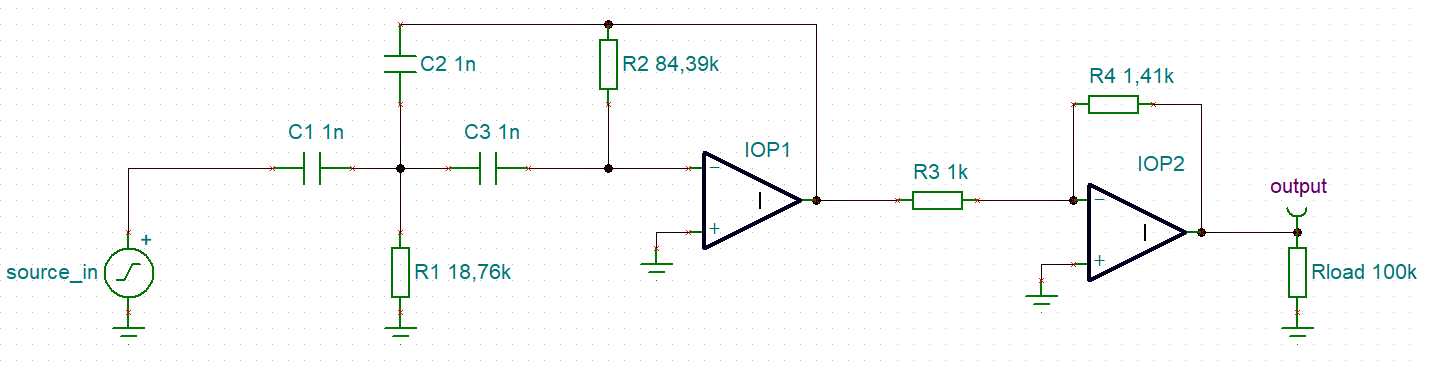
\includegraphics[width=0.8\textwidth]{rauh1}}
	\caption{Схема рауха інвертуючого ФВЧ-2 та масштабуючого підсилювача з розрахованими номіналами}
	\end{figure}

\clearpage
\begin{center}
\fbox{8}
\end{center}
	Побудуймо АЧХ та ФЧХ нашого фільтру:
	\begin{figure}[h]

	{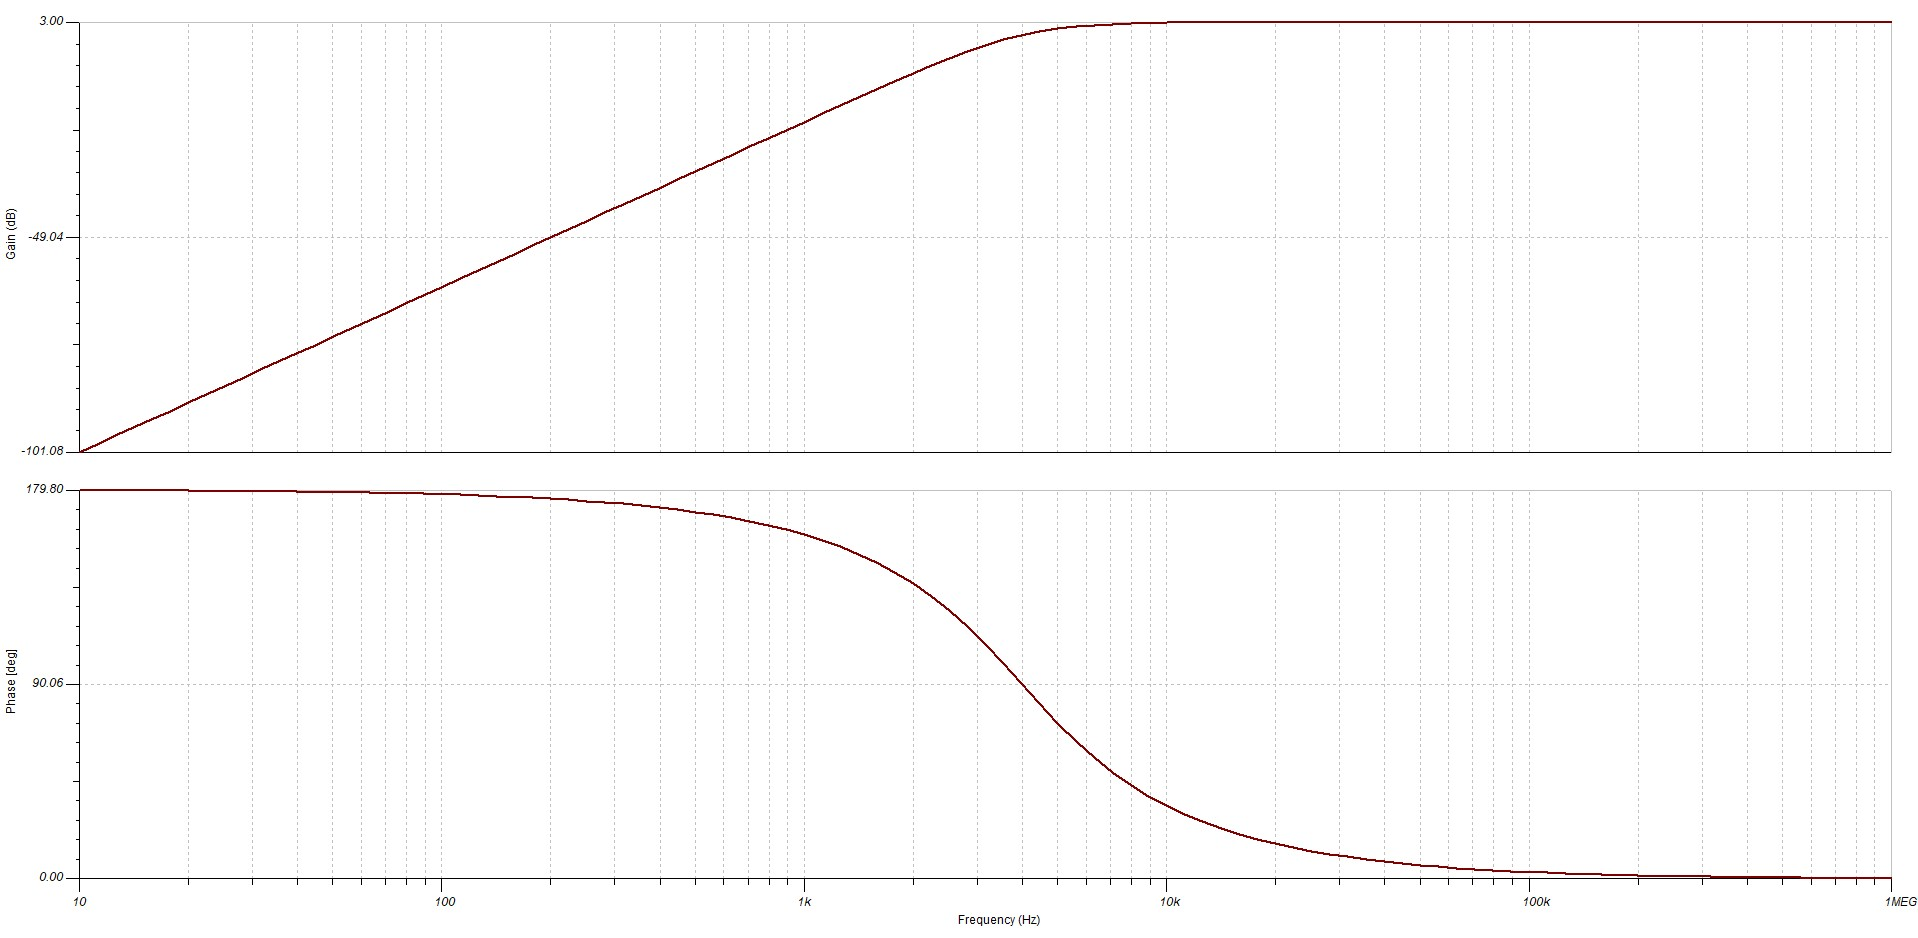
\includegraphics[width=\textwidth]{req}}
	\caption{АЧХ (зверху) та ФЧХ (знизу) фільтра}
	\end{figure}
	\newpage
	Розглянемо більш детально амплітудну характеристику:
	\begin{figure}[h]

	{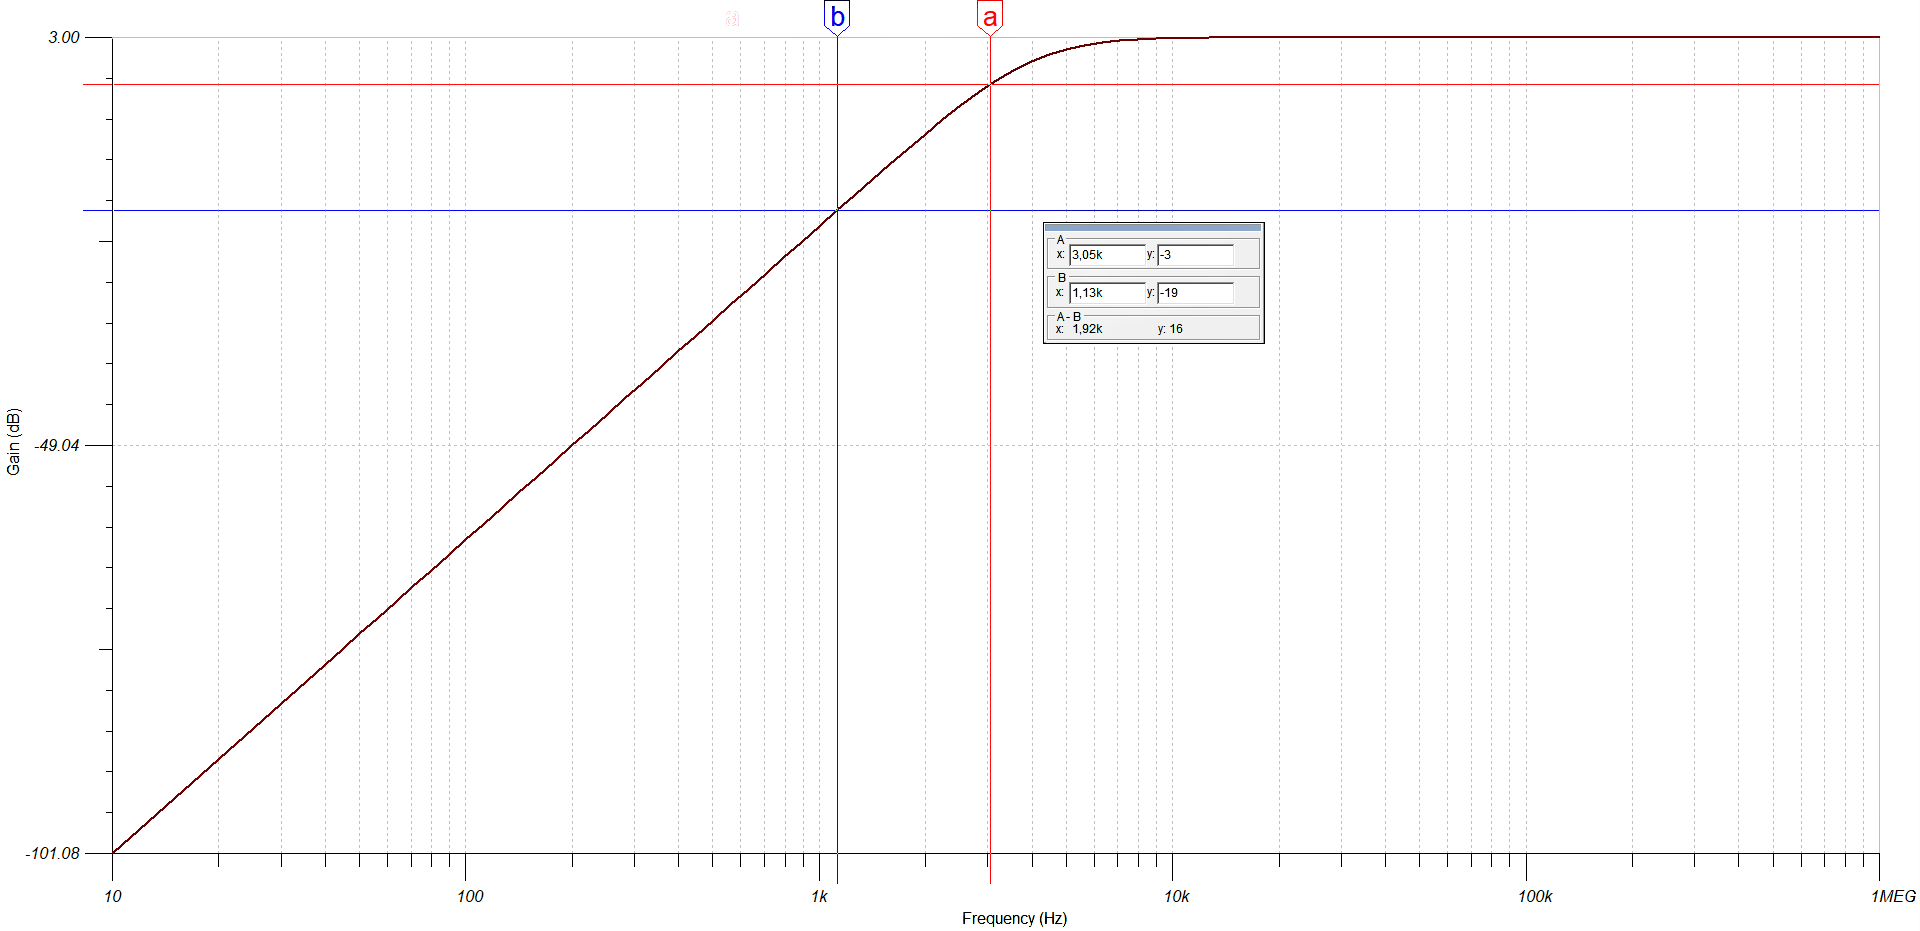
\includegraphics[width=\textwidth]{amplitude}}
	\caption{АЧХ фільтра}
	\end{figure}

	В специфікації було сказано, що коефіцієнт передачі в смузі пропускання має становити 3 дБ, що ми і можемо спостерігати на графіку- підсилення в 3 дБ наявне. Розглянемо вертикальний червоний маркер $a$, що відтинає на осі $Gain (dB)$ рівень -3 дБ. Як ми пам'ятаємо з умов специфікації, рівень пульсації в смузі пропускання становить 6 дБ, тобто значеня в -3 дБ (3-6) має спостерігатись на частоті $f_p=4$ кГц. На графіку ж значення $f_p=3,05$, тобто відносна похибка $\delta$ склала $31,15\%$. Розглянувши вертикальний червоний маркер $b$, що відтинає рівень -19 дБ, ми бачимо що фактична частота $f_s$ складає 1,13 кГц, що доволі непогано відповідає умовам специфікації ($f_s=1,33$ кГц), відносна похибка тут складає всього $17,7\%$.\\

	Розглянувши ФЧХ нашого фільтру, ми бачимо, що вона є зеркально протилежною до теоретичних викладок, але це можна пояснити наявністю в ланці додаткового інвертуючого масштабуючого підсилювача.  










\end{document}
